\subsection{Création des ressources}
\subsubsection{Conception du modèle 3d et des textures}
La map du jeu, représentant le bâtiment Claude Chappe et ses
environs, a été créée en plusieurs étapes via Blender : \\ \\
\textbf{- Modélisation 3D des modèles :} \\
\\
On utilise des objets préfabriqués de Blender, modifiables
grâce à divers outils pour obtenir les formes désirées (ex :
transformation d'un cube en mur ou en porte comme on le voit
figure ~\ref{fig:cube-base} et ~\ref{fig:cube-modif}). Nous
avons d'abord modélisé la structure de base du bâtiment, puis
ajouté des éléments exclusifs au jeu, comme des trous dans le
sol et les murs pour un parcours de poursuite, ainsi que trois
salles secrètes avec des ordinateurs pour les mini-jeux.\\

\textbf{- Normals :} \\\\
Les normales définissent l'orientation des faces des objets et
influencent l'effet de la lumière. Bien que généralement correctes
par défaut, il est parfois nécessaire de les ajuster pour éviter
des erreurs d'affichage. \\

\textbf{- Texturage :} \\ \\
Une fois les objets modélisés, ils sont texturés en utilisant des
textures d’image ou des couleurs unies, compatibles avec le
moteur 3D. Par exemple, une porte est texturée en rouge uni,
tandis que les murs utilisent une texture image de plastique
gris/blanc.\\

\textbf{- Séparation des zones :} \\

Les objets sont regroupés en "collections" selon leur emplacement
(amphithéâtre, couloirs, salles de classe, etc.), ce qui facilite
leur exportation en fichiers .obj distincts et optimise le
chargement des ressources dans le moteur.\\

\textbf{- Optimisation des modèles et textures :} \\

Les erreurs de modélisation sont corrigées pour garantir une
bonne intégration. Les UV Maps des textures sont ajustées pour
assurer un affichage correct après l'exportation.\\

\textbf{- Exportation :} \\

Les objets d’une zone sont fusionnés (JOIN) pour simplifier
l’importation dans le moteur (un seul objet au lieu de plusieurs
centaines). On les exporte ensuite en .obj et .mtl (textures), en
veillant à inclure toutes les images de textures nécessaires.

\begin{figure}
    \centering
    \begin{minipage}{0.49\linewidth}
        \centering
        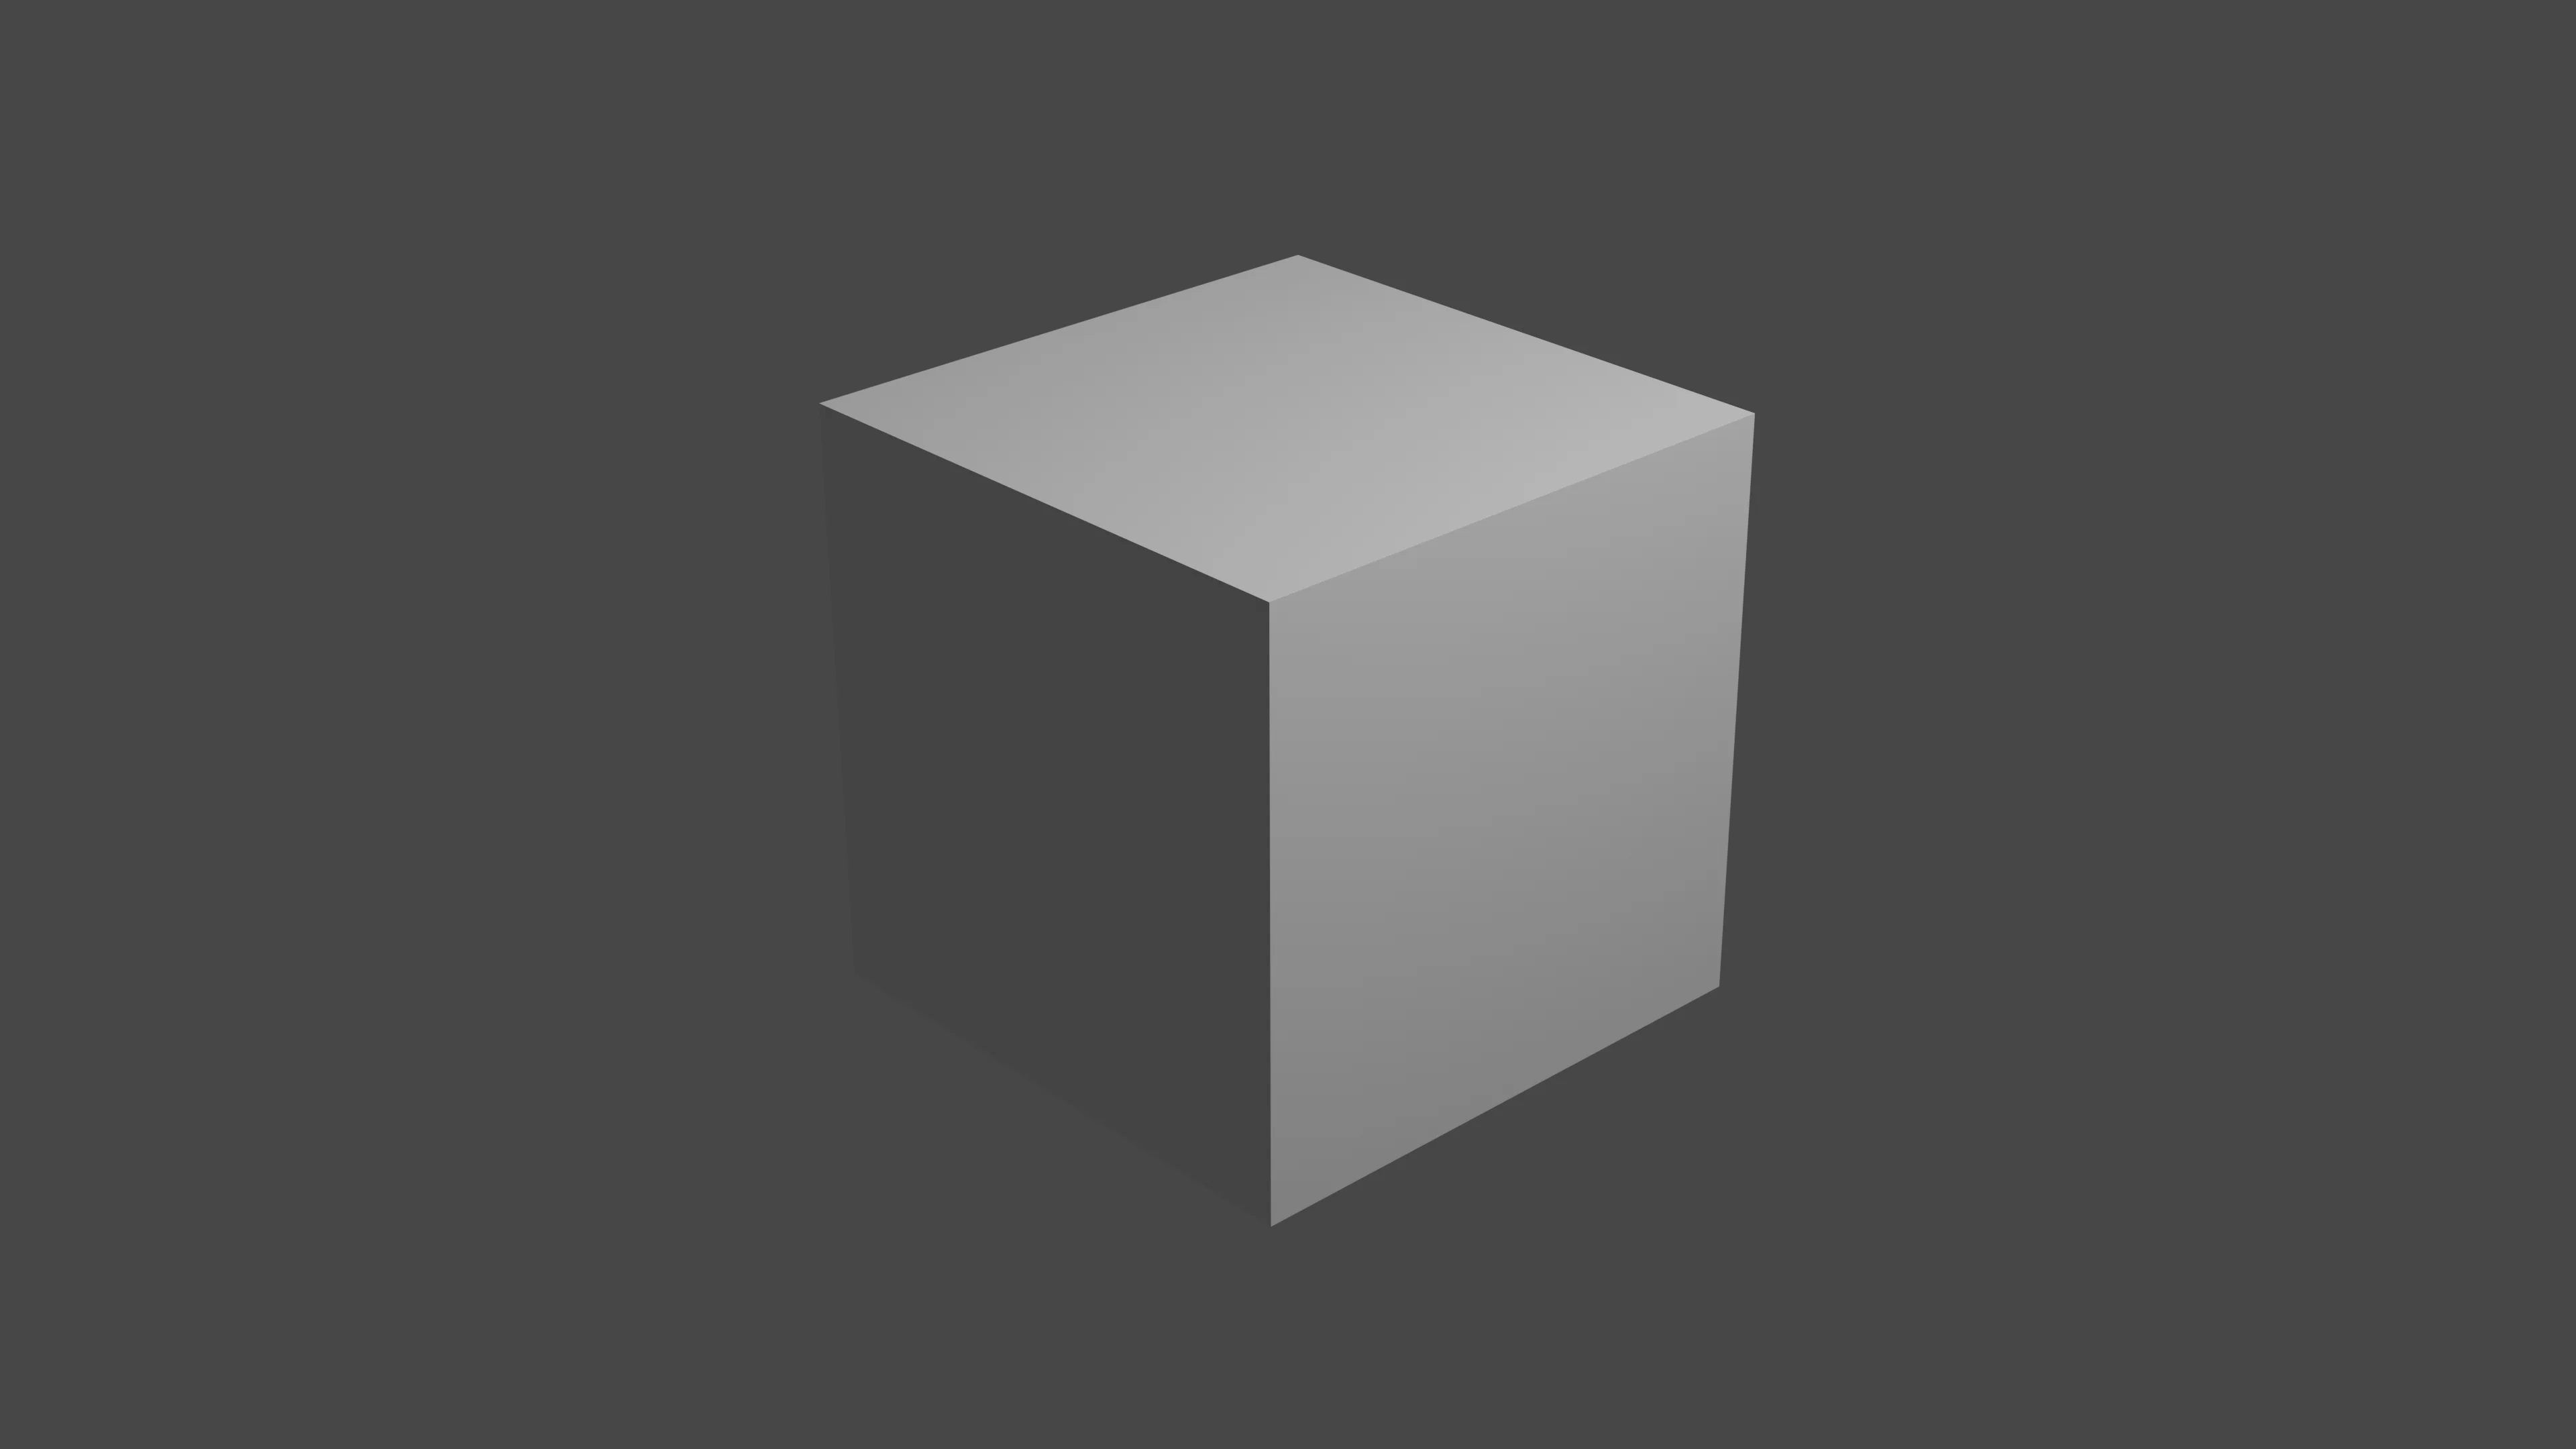
\includegraphics[width=\linewidth]{images/base_cube.png}
        \caption{Cube de base Blender}
        \label{fig:cube-base}
    \end{minipage}
    \hfill
    \begin{minipage}{0.49\linewidth}
        \centering
        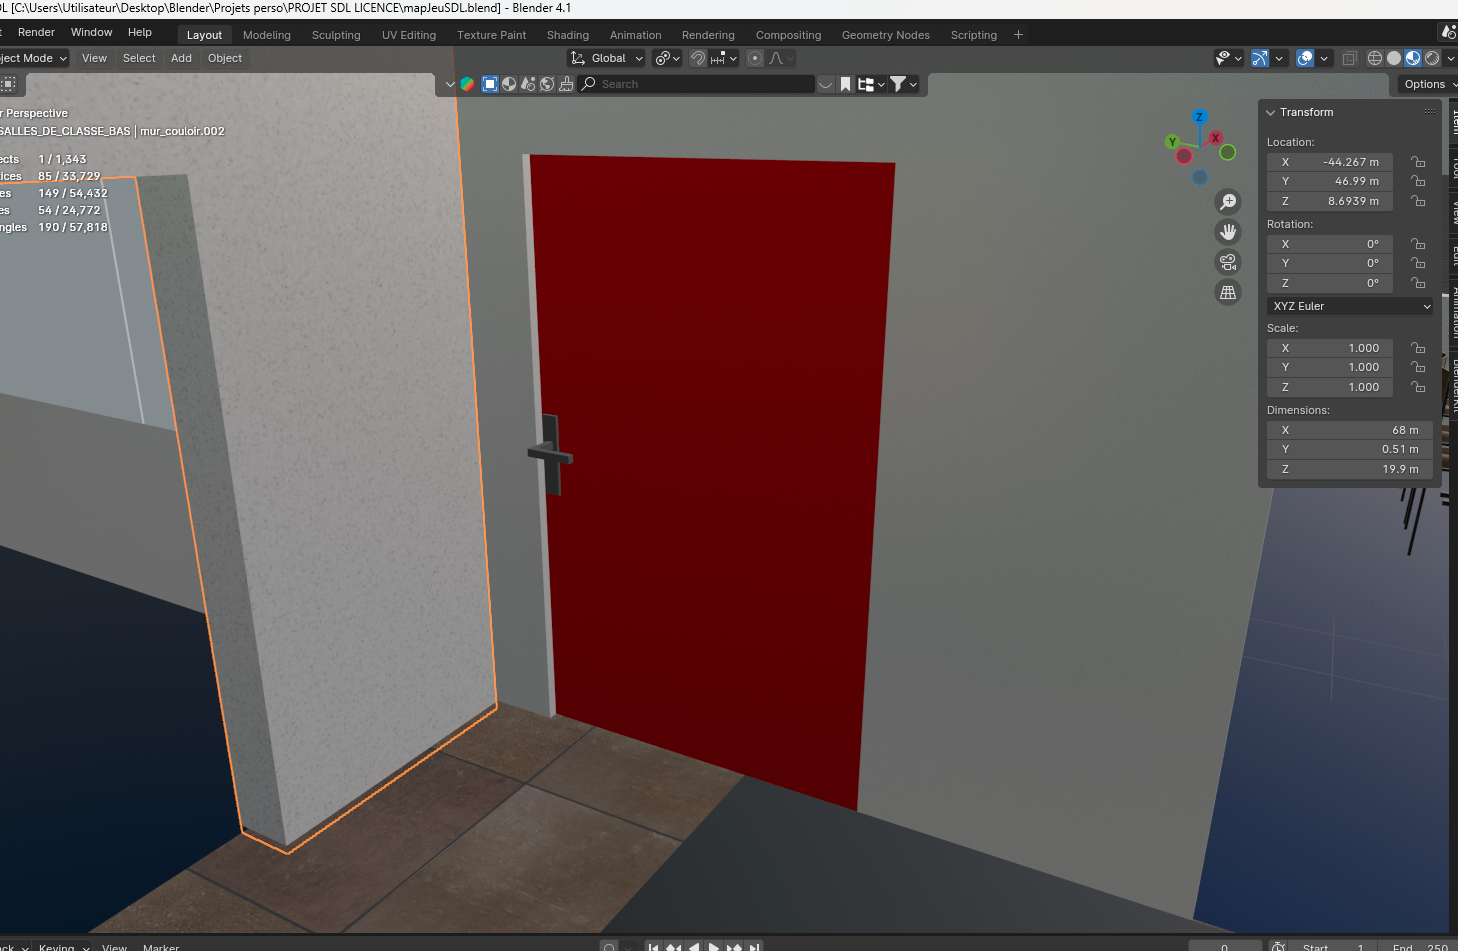
\includegraphics[width=\linewidth]{images/cubemodif.png}
        \caption{Cubes modifiés en divers objets}
        \label{fig:cube-modif}
    \end{minipage}
\end{figure}
\subsubsection{Conception des musiques et effets sonores}

Les musiques et les effets sonores sont tous les deux composés
sur le logiciel FL Studio.\\\\
\textbf{- Conception des musiques :}\\\\
À partir de sons déjà existants (libres de droits), on les
utilise en les modifiant (ou non), pour en faire des mélodies
(à l'aide d'un clavier synthétiseur), des boucles de divers instruments,
bref créer une musique.\\\\
\textbf{- Conception des effets sonores :}\\\\
Pour les effets sonores, on utilise à nouveau des sons déjà
existants, évidemment sans faire des mélodies cette fois. On les
modifie à travers divers plugins du logiciel (pitch grave/aigu,
réverbération, etc.).\\
Vous trouverez en annexe un exemple de composition musicale (voir figure \ref{fig:flstudio.png}).